\documentclass{article}
\usepackage{inputenc}
\usepackage{setspace}
\usepackage[margin=0.75in]{geometry}
\usepackage[style=numeric]{biblatex}
\addbibresource{../bibs/ref.bib}
\usepackage{float}
\usepackage{graphicx}
\graphicspath{ {./images/} }


\onehalfspace
\setlength{\parindent}{0pt}
\setlength{\parskip}{1em}



\begin{document}

\begin{center}
  \LARGE{\textbf{Real-world Functional Programming}} \\
  \Large{Coursework Part II Report} \\
  \normalsize{14274056 Junsong Yang (psyjy3)} \\
  \today
\end{center}


\begin{normalsize}
  \section{Task II.1}

  \begin{figure}[H]

    \begin{minipage}[b]{0.48\linewidth}
      \centering
      \centerline{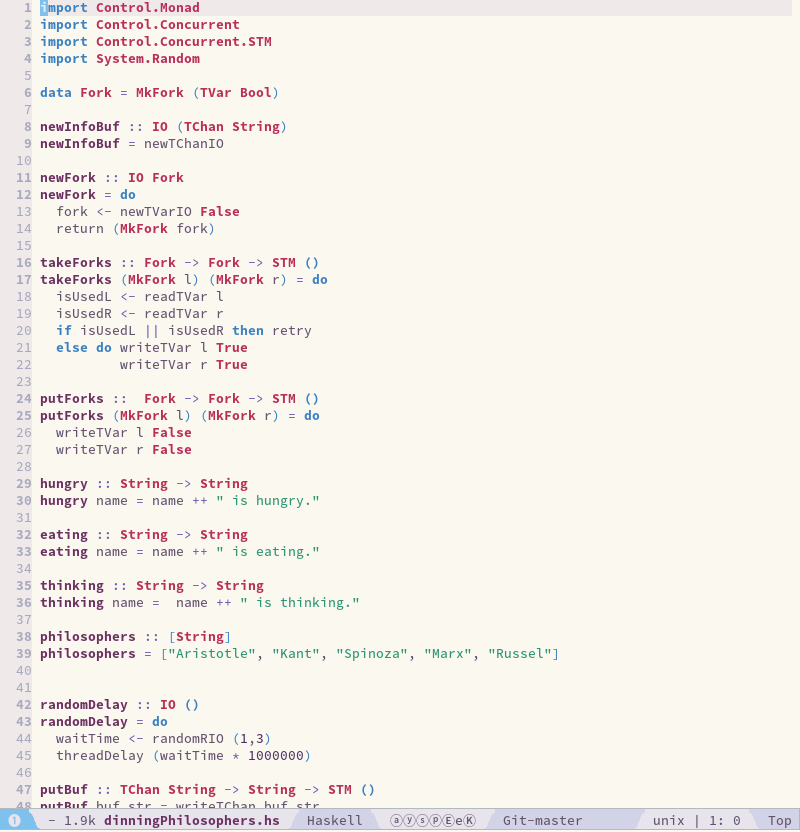
\includegraphics[width=8.5cm]{dinning1}}
      \centerline{ (a) Dinning Phhilosopher Part I}\medskip
    \end{minipage}
    \hfill
    \begin{minipage}[b]{0.48\linewidth}
      \centering
      \centerline{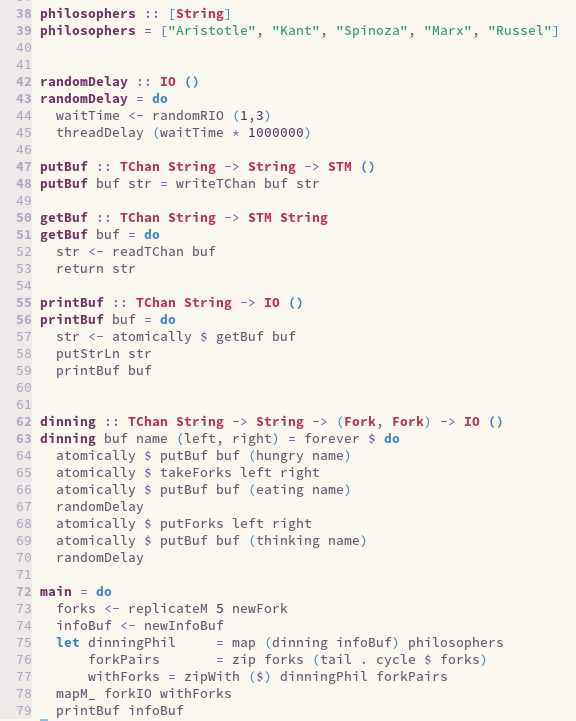
\includegraphics[width=8.5cm, height=12.5cm]{dinning2}}
      \centerline{ (b) Dinning Phhilosopher Part II }\medskip
    \end{minipage}
    \caption{Dinning Phhilosopher}
    \label{fig:dinning}
  \end{figure}

  Figure \ref{fig:dinning} contains two figures that show the full
  implementation of dinning philosopher using STM. Starting with figure
  \ref{fig:dinning} (a), the Fork type is defined with a constructor called
  MkFork which take a TVar with a Bool as a input. If the boolean inside the
  TVar is false then this fork is available to be used otherwise this fork is
  already taken. The newInfoBuf function will return a TChan with String wrapped
  in IO monad to be used later to store logs that indicate the running state of
  each thread. The newFork function will return a Fork wrapped in IO monad with
  the boolean value set to false.

  The next two function takeForks and putForks are related to require and
  release resources. The takeForks function takes two Fork as input. This
  function will first check if the two Forks are both available. The two Forks
  can only be used if they are both available as the same time. Otherwise, this
  function will keep retrying untill both Forks can be required. The putForks
  function is simple just release the two Forks by setting the boolean to true.

  The next three functions hungry, eating, thinking are just dummy function that
  concatenate the name of philosopher with corresponding information. These
  information will later be put into the infoBuf(TChan String). The names of
  philosophers are defined as a list of string as figure \ref{fig:dinning} (b)
  shows.

  The randomDelay will call threadDelay to delay the running thread randomly
  from 1 to 3 seconds. The next three functions, putBuf, getBuf printBuf are
  operations related to the infoBuf(TChan String) that is used to store the logs
  for running thread. The putBuf function will just store string to the
  infoBuf(TChan String), the getBuf function will return the string stored in
  TChan and wrap in STM monad. The printBuf will just print the string stored in
  TChan.

  The dinning function is contains the implementation of dinning philosophers.
  This function takes a TChan String(used to store logs), a string(indicates
  philosopher's names), and a pair of Fork as input. This function will first
  store a log in the TChan that indicates the philosopher is hungry. Then, this
  function will trying to acquire the Fork using takeForks function. If the
  forks are acquired successfully, another log will be stored in the TChan that
  suggests the philosopher is eating. Followed by a random delay from 1 to 3
  seconds, the forks will be released using putForks function and corresponding
  log will be put into the TChan. Finally, the function ended with another
  random delay.

  The main function will first initialise 5 Forks using newFork function and a
  infoBuf using newInfoBuf functions. Then the philosophers' name will be
  bundled with the dinning function using map. Then, a infinite list of pair of
  forks will be generated such that each fork in the pair is distinct from the
  other. Followed by coupling pairs of forks with the dinning function, a list
  of runnable functions is made. Finally, the main function will run those
  function by mapping forkIO function to the runnable dinning functions while
  the printBuf function is called to print the logs of those running thread.

   \begin{figure}[H]

    \begin{minipage}[b]{0.24\linewidth}
      \centering
      \centerline{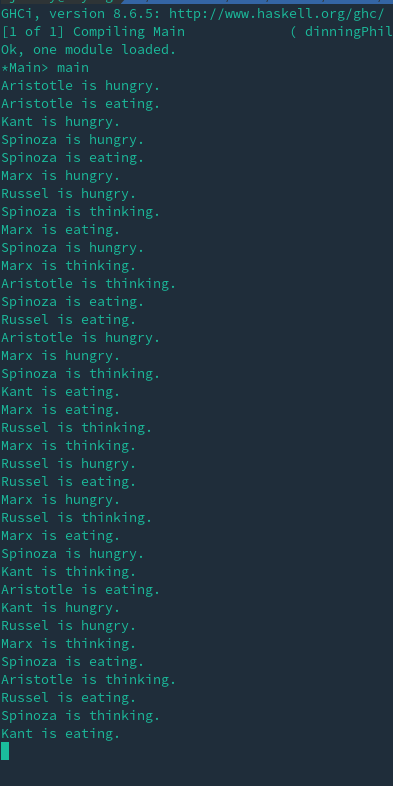
\includegraphics[width=4.0cm]{dinning10s}}
      \centerline{ (a) running at 10s}\medskip
    \end{minipage}
    \hfill
    \begin{minipage}[b]{0.24\linewidth}
      \centering
      \centerline{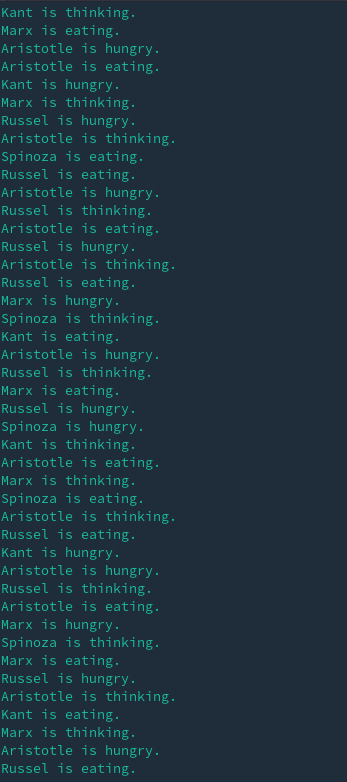
\includegraphics[width=4.0cm]{dinngin1m}}
      \centerline{ (b) running at 1m}\medskip
    \end{minipage}
    \hfill
    \begin{minipage}[b]{0.24\linewidth}
      \centering
      \centerline{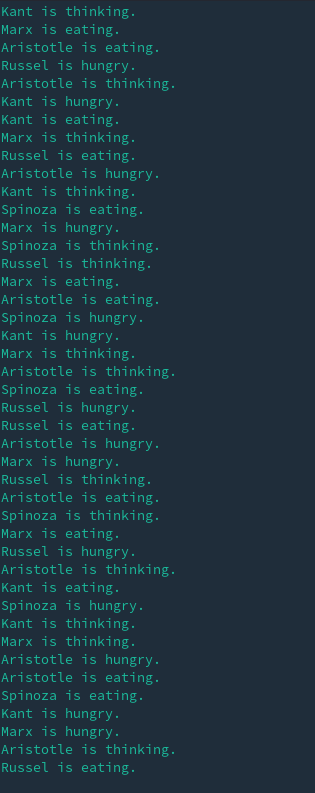
\includegraphics[width=4.0cm]{dinning2m}}
      \centerline{ (c) running at 2m}\medskip
    \end{minipage}
    \hfill
    \begin{minipage}[b]{0.24\linewidth}
      \centering
      \centerline{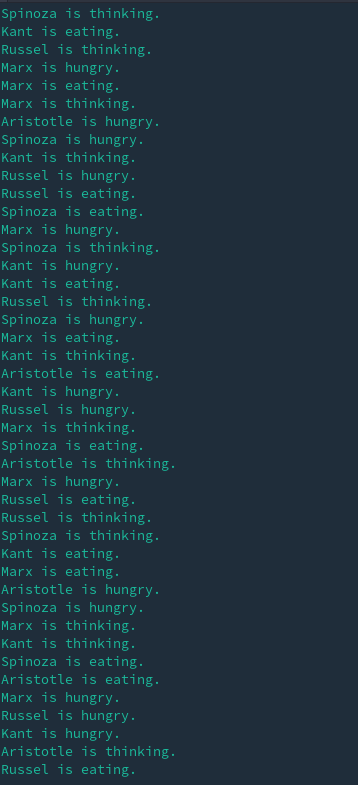
\includegraphics[width=4.0cm]{dinning4m}}
      \centerline{ (b) running at 4m}\medskip
    \end{minipage}

    \caption{Dinning Philosopher Running at Defferent Point of Time}
    \label{fig:drunning}
  \end{figure}

  Figure \ref{fig:drunning} contains four figures that shows this implementation
  running non-stop for four minutes. These sample output of the running program
  suggests that this implementation is working and without deadlocks. The main
  reason that this implementation is free of deadlocks is that it does not use
  locks at all and also this implementation uses STM which allows the threads
  running without the knowledge of the global environment. Giving two forks,
  each thread simple keep trying to acquired them at the same time until success.
  In this way, deadlocks can be avoid as resources will be acquired only until
  they are available. In contrast, if a thread acquired partially available and
  wait until other resource is available then deadlocks may easily occur.

  There are other solutions like resource hierarchy solution and arbitrator
  solution available for this problem. The resource hierarchy solution follows
  conventions that all forks are acquired in order and only one philosopher can
  pick up the fork in the highest order. This solution require that all
  resources are known to all the philosophers. But this is often hard to achieve in
  real-world use cases which makes this solution impractical. As for the
  arbitrator solution, resource acquisition is controlled by a arbitrator instead
  of philosophers. While philosophers can put down forks at any time, the
  permission of picking up forks is controlled by the arbitrator and the
  arbitrator will grant the permission to only one philosophers at a time. One
  obvious issue for this solution is the permission control. All philosophers
  have to wait for the permission from the arbitrator even if there are forks
  available. This issue would often cause efficiency problems.

  Comparing to those two solutions, STM solution is free of deadlocks and also
  the code is simple to write and expressive. But the STM solution is suffering
  from time penalty for committing atomic transactions. Also, one limitation of
  STM need to be considered is that all the operations that can be performed by
  STM must be revertible. Despite its disadvantages and limits, STM is justified
  by its benefits.

  \section{Task II.2}
  Before the explanation of this implementation, the capabilities of this
  calculator will be introduced. The features supported by this calculator are:
  \begin{itemize}
  \item{Handle at least 10-digit integers}
  \item{Support addition, subtraction, multiplication, and division}
  \item{Allow the sign to be changed (+/-)}
  \item{Allow the calculator to be reset (C) as well as clearing the last
      entry (CE)}
  \item{Support calculations with decimal fractions (decimal point)}
  \item{Support standard precedence rules among the arithmetic operations
  along with parentheses for grouping}
  \item{Have a clearly structured implementation making use of functional
      reactive programming}
  \end{itemize}

  
  \begin{figure}[H]
    \centering
    \centerline{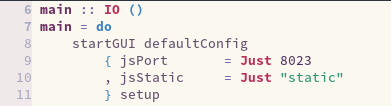
\includegraphics[scale=0.4]{calcmain}}
    \caption{Calculator Main Function}
    \label{fig:calcmain}
  \end{figure}

  Figure \ref{fig:calcmain} show the main function of the calculator. This
  function is adopted from the examples provided by the threepenny library.

  The setup function is where the logic and ui are defined.

    \begin{figure}[H]

    \begin{minipage}[b]{0.48\linewidth}
      \centering
      \centerline{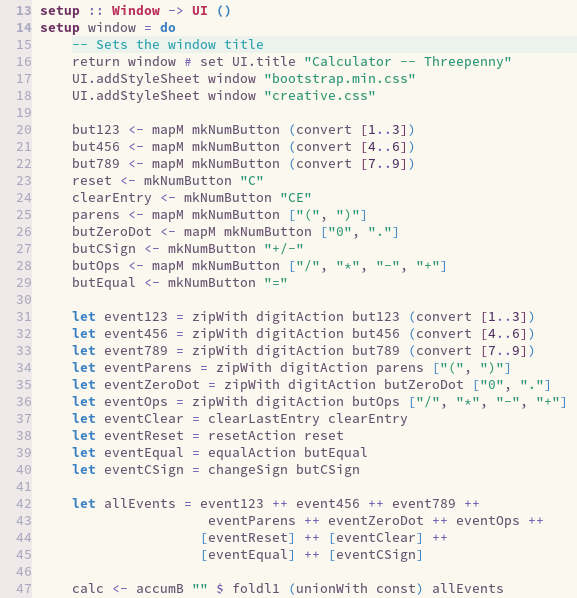
\includegraphics[width=8.5cm]{calcsetup1}}
      \centerline{ (a) Part I}\medskip
    \end{minipage}
    \hfill
    \begin{minipage}[b]{0.48\linewidth}
      \centering
      \centerline{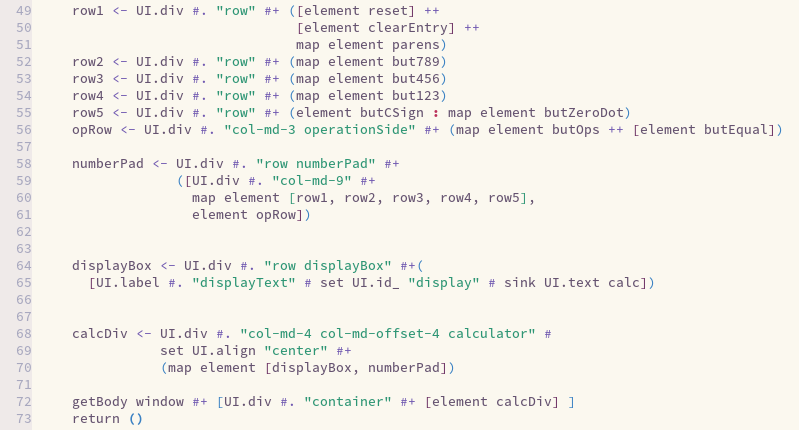
\includegraphics[width=8.5cm,height=5.5cm]{calcsetup2}}
      \centerline{ (b) Part II }\medskip
    \end{minipage}
    \caption{Calculator Setup Function}
    \label{fig:dinning}
  \end{figure}


  css \footnote[]{https://github.com/xxczaki/calculator.js/blob/5d8ec0901e3503a6480d086df0d8e55c39908cdc/css/creative.css}
  
  \begin{figure}[H]
    \centering
    \centerline{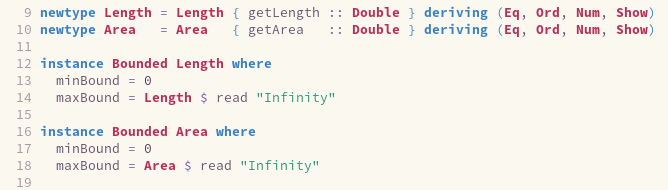
\includegraphics[scale=0.4]{StatsBonusBound}}
    \caption{newtype Bounded}
    \label{fig:bounded}
  \end{figure}

  
  \begin{figure}[H]

    \begin{minipage}[b]{0.48\linewidth}
      \centering
      \centerline{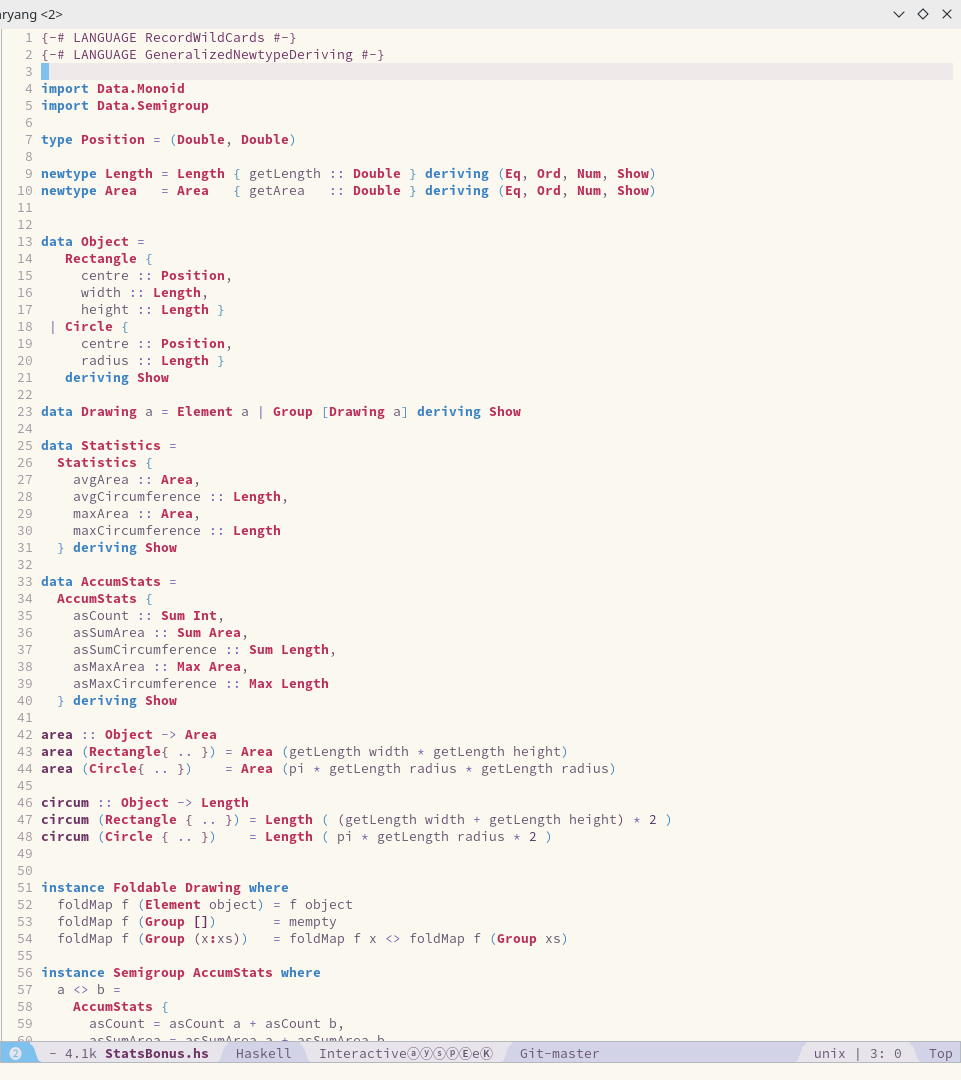
\includegraphics[width=8.0cm]{StatsBonus}}
      % \vspace{1.5cm}
      \centerline{ (a) Recursive Statistics for newtype}\medskip
    \end{minipage}
    \hfill
    \begin{minipage}[b]{0.48\linewidth}
      \centering
      \centerline{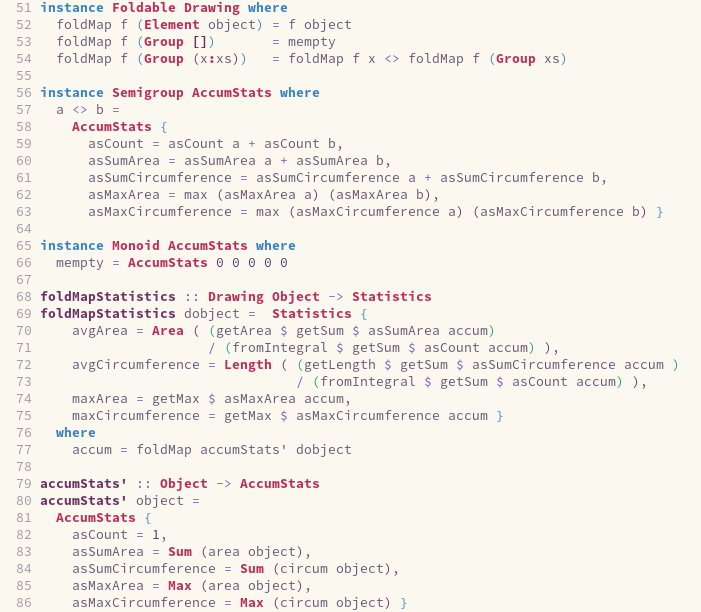
\includegraphics[width=8.0cm]{StatsBonusFoldMap}}
      % \vspace{1.5cm}
      \centerline{ (b) Statistics using foldMap for newtype}\medskip
    \end{minipage}
    % 
    \caption{TaskI.5 3}
    \label{fig:taskI.5.3}
    % 
  \end{figure}

  
\end{document}

